\subsection{Cavity measurements}\label{sec:cavity_measurements}

\subsubsection{Determining the cavity length from the FSR}

\begin{figure}[h!]
    \centering
    \begin{subfigure}[b]{0.45\textwidth}
        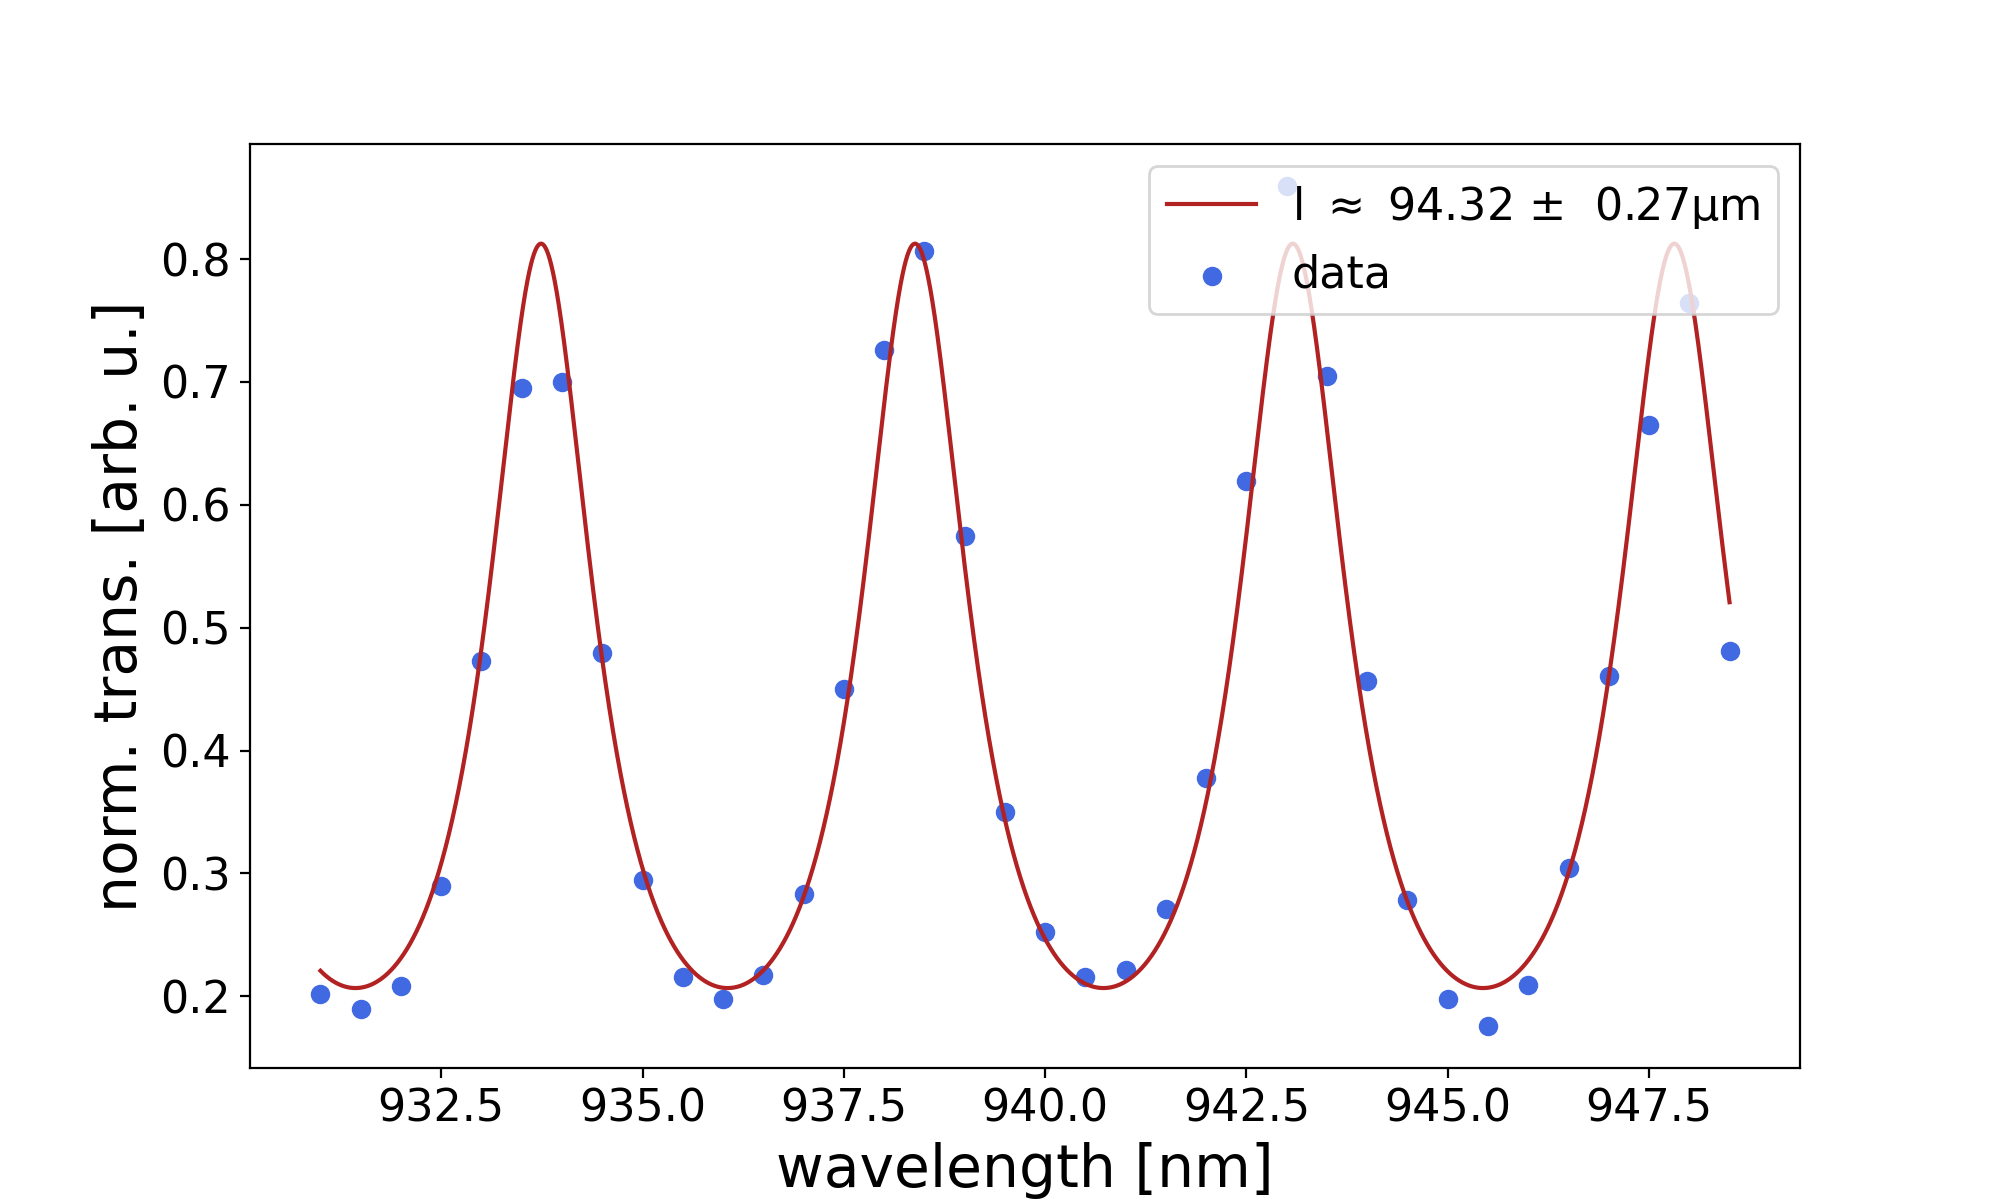
\includegraphics[width=\textwidth]{figures/length_from_fsr_example_100um.png}
        \caption{}
        \label{fig:100um_FSR}
    \end{subfigure}
    \begin{subfigure}[b]{0.45\textwidth}
        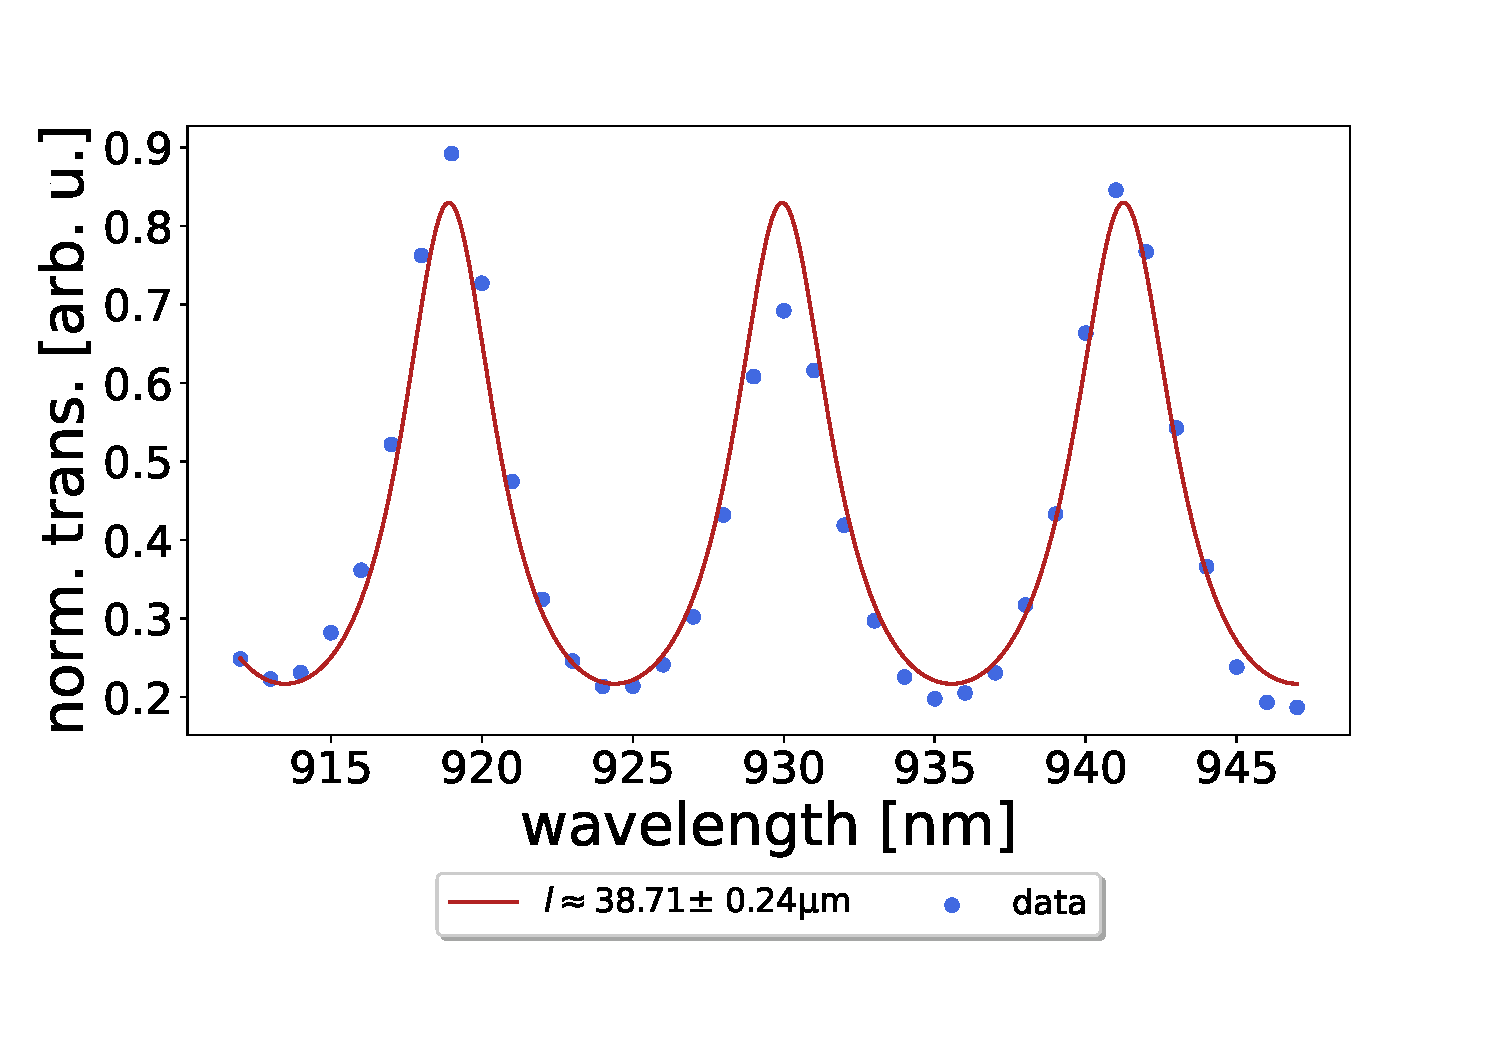
\includegraphics[width=\textwidth]{figures/length_from_fsr_example_40um.pdf}
        \caption{}
        \label{fig:40um_FSR}
    \end{subfigure}
    \caption{}
    \label{fig:length_from_long_scan_example}    
\end{figure}

Figures: 
\begin{itemize}
    \item Linewidth as a function of "time" - to see the reduction of the linewidth as the piezo reaches an equilibrium where any time-dependent drift is reduced. 
\end{itemize}

\subsubsection{Normalization}

\subsubsection{Single fano cavity characterization} 

\subsubsection{Aligning the cavity}

\begin{figure}[h!]
    \centering
    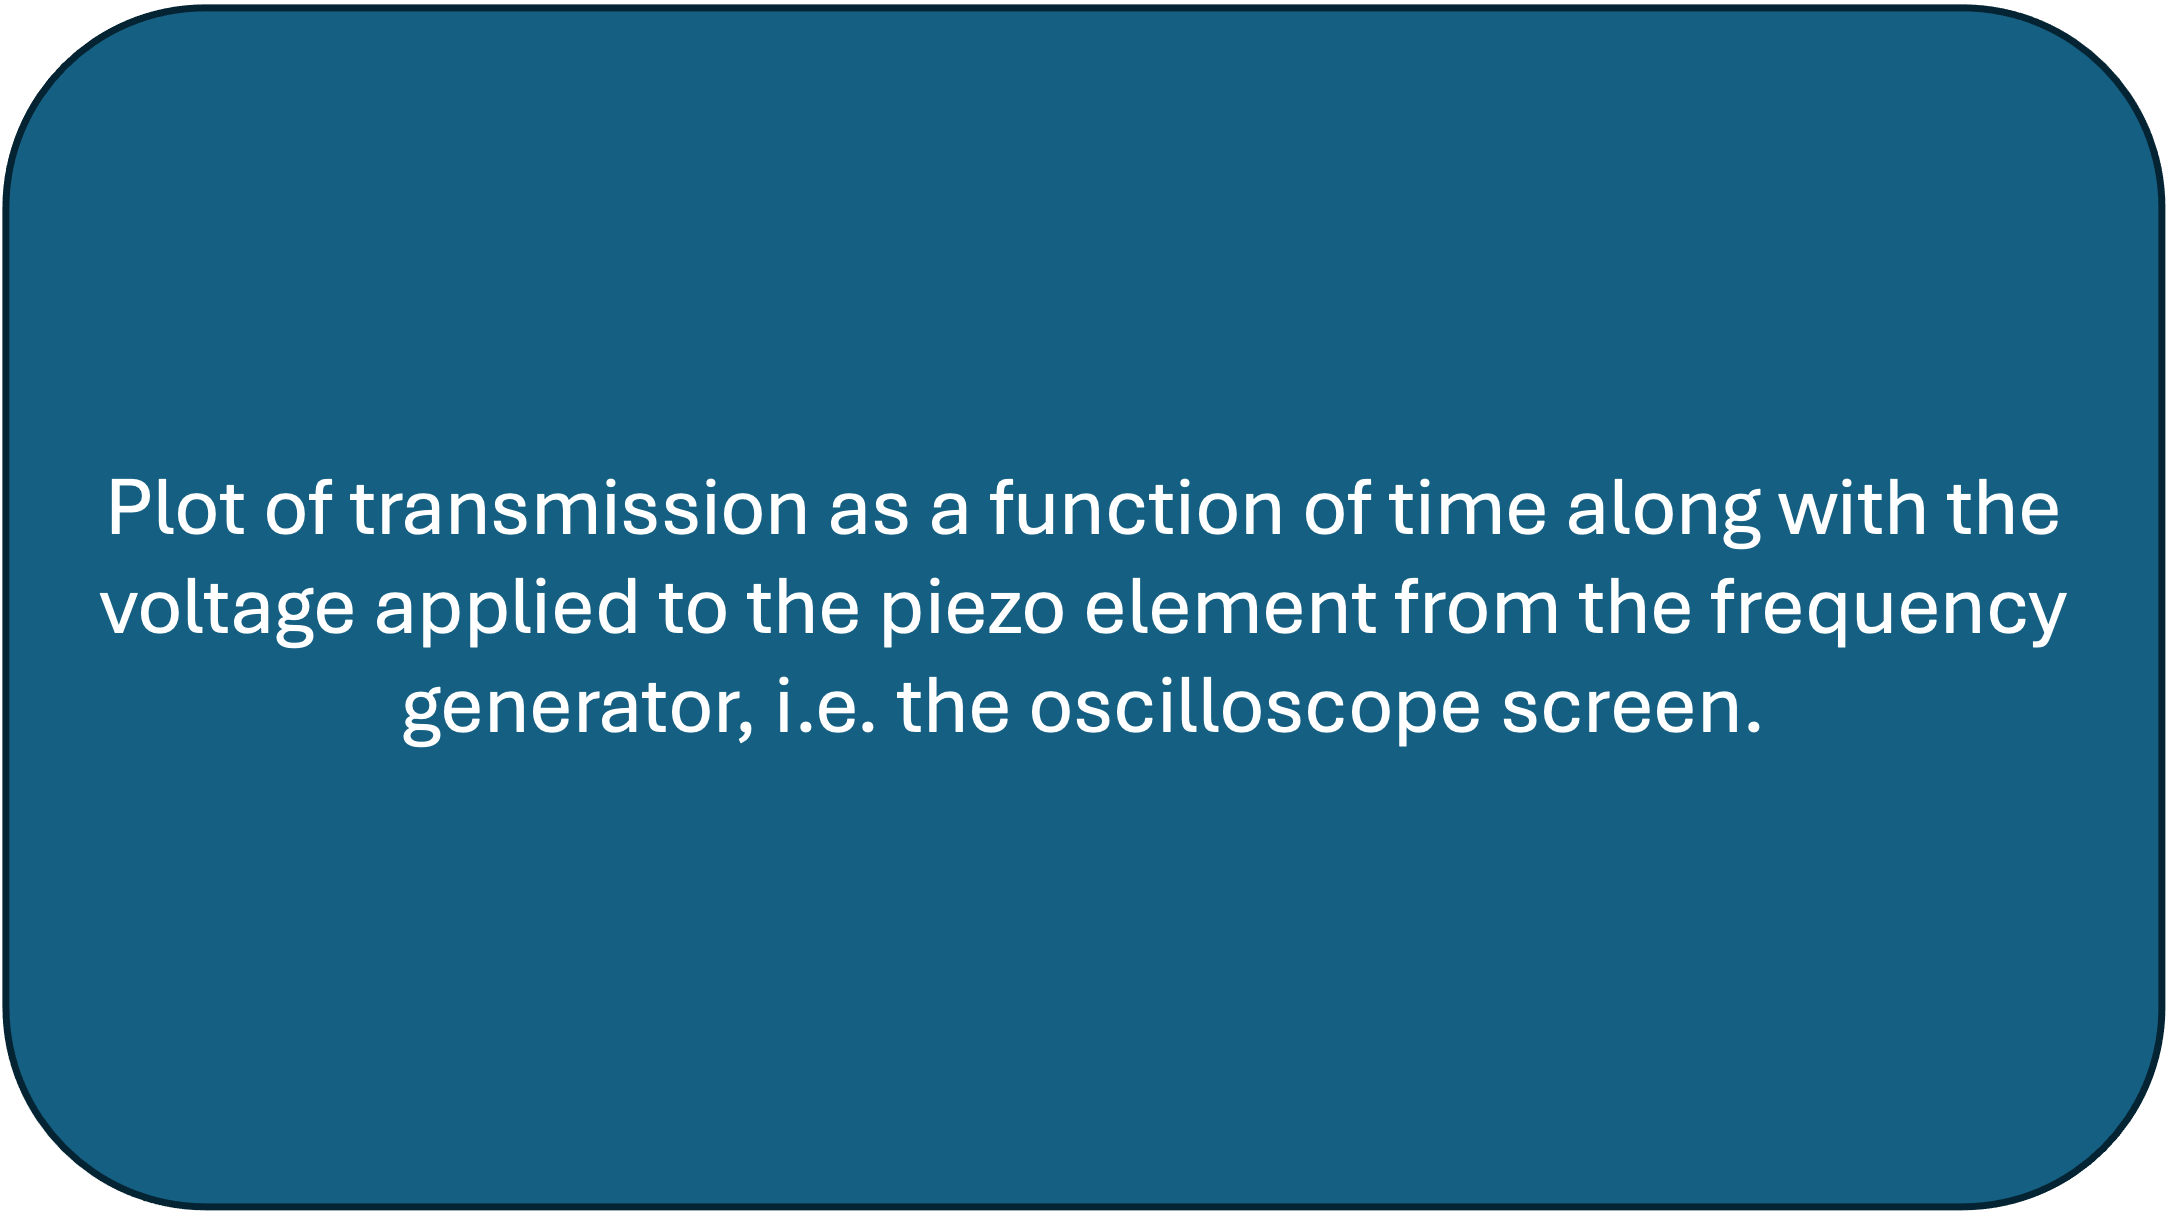
\includegraphics[width=0.6\textwidth]{figures/placerholder.png}
    \caption{}
    \label{fig:placeholder}
\end{figure}

Incluce: 
\begin{itemize}
    \item Scan for optimal cavity length
    \item Measure the spectral linewidth
    \item 
\end{itemize}

\subsubsection{Double fano cavity characterization}

\subsubsection{Off-resonance Fabry-Perot cavity (alignment technique)}

\subsubsection{Centering of the top grating (pinhole method)}

\subsection{Parallelism study (deviation from normal incident)}

